	\newpage
\section{Testowanie}	%5
%Opisujemy testy, sprawdzamy czy nie generuje błędów.

\subsection{Testowanie latarki.}

\begin{tabela}
	{Testowanie latarki}	%opis w spisie tabel
	{Testowanie latarki}	%opis przy tabeli
	{
		\begin{tabular}{|c|c|c|c|c|} \hline
			lp & Zadania do przetestowania & Tak & Nie \\ \hline
			1 & Latarka po naciśnięciu na guzik włączyła się & X & ~ \\ \hline
			2 & Po włączeniu latarki, guzik zmienia kolor na zielony & X & ~ \\ \hline
			3 & Latarka po naciśnięciu na guzik wyłączyła się & X & ~ \\ \hline
			4 & Po wyłączeniu latarki, guzik zmienia kolor na czerwony & X & ~ \\ \hline
		\end{tabular}	}
	\label{tab:tablica001}
\end{tabela}

Obrazek \ref{rys:latarka} przedstawia zrzuty ekranu potwierdzające pomyślny przebieg testu.

\begin{figure}[!hbt]
	\begin{center}
		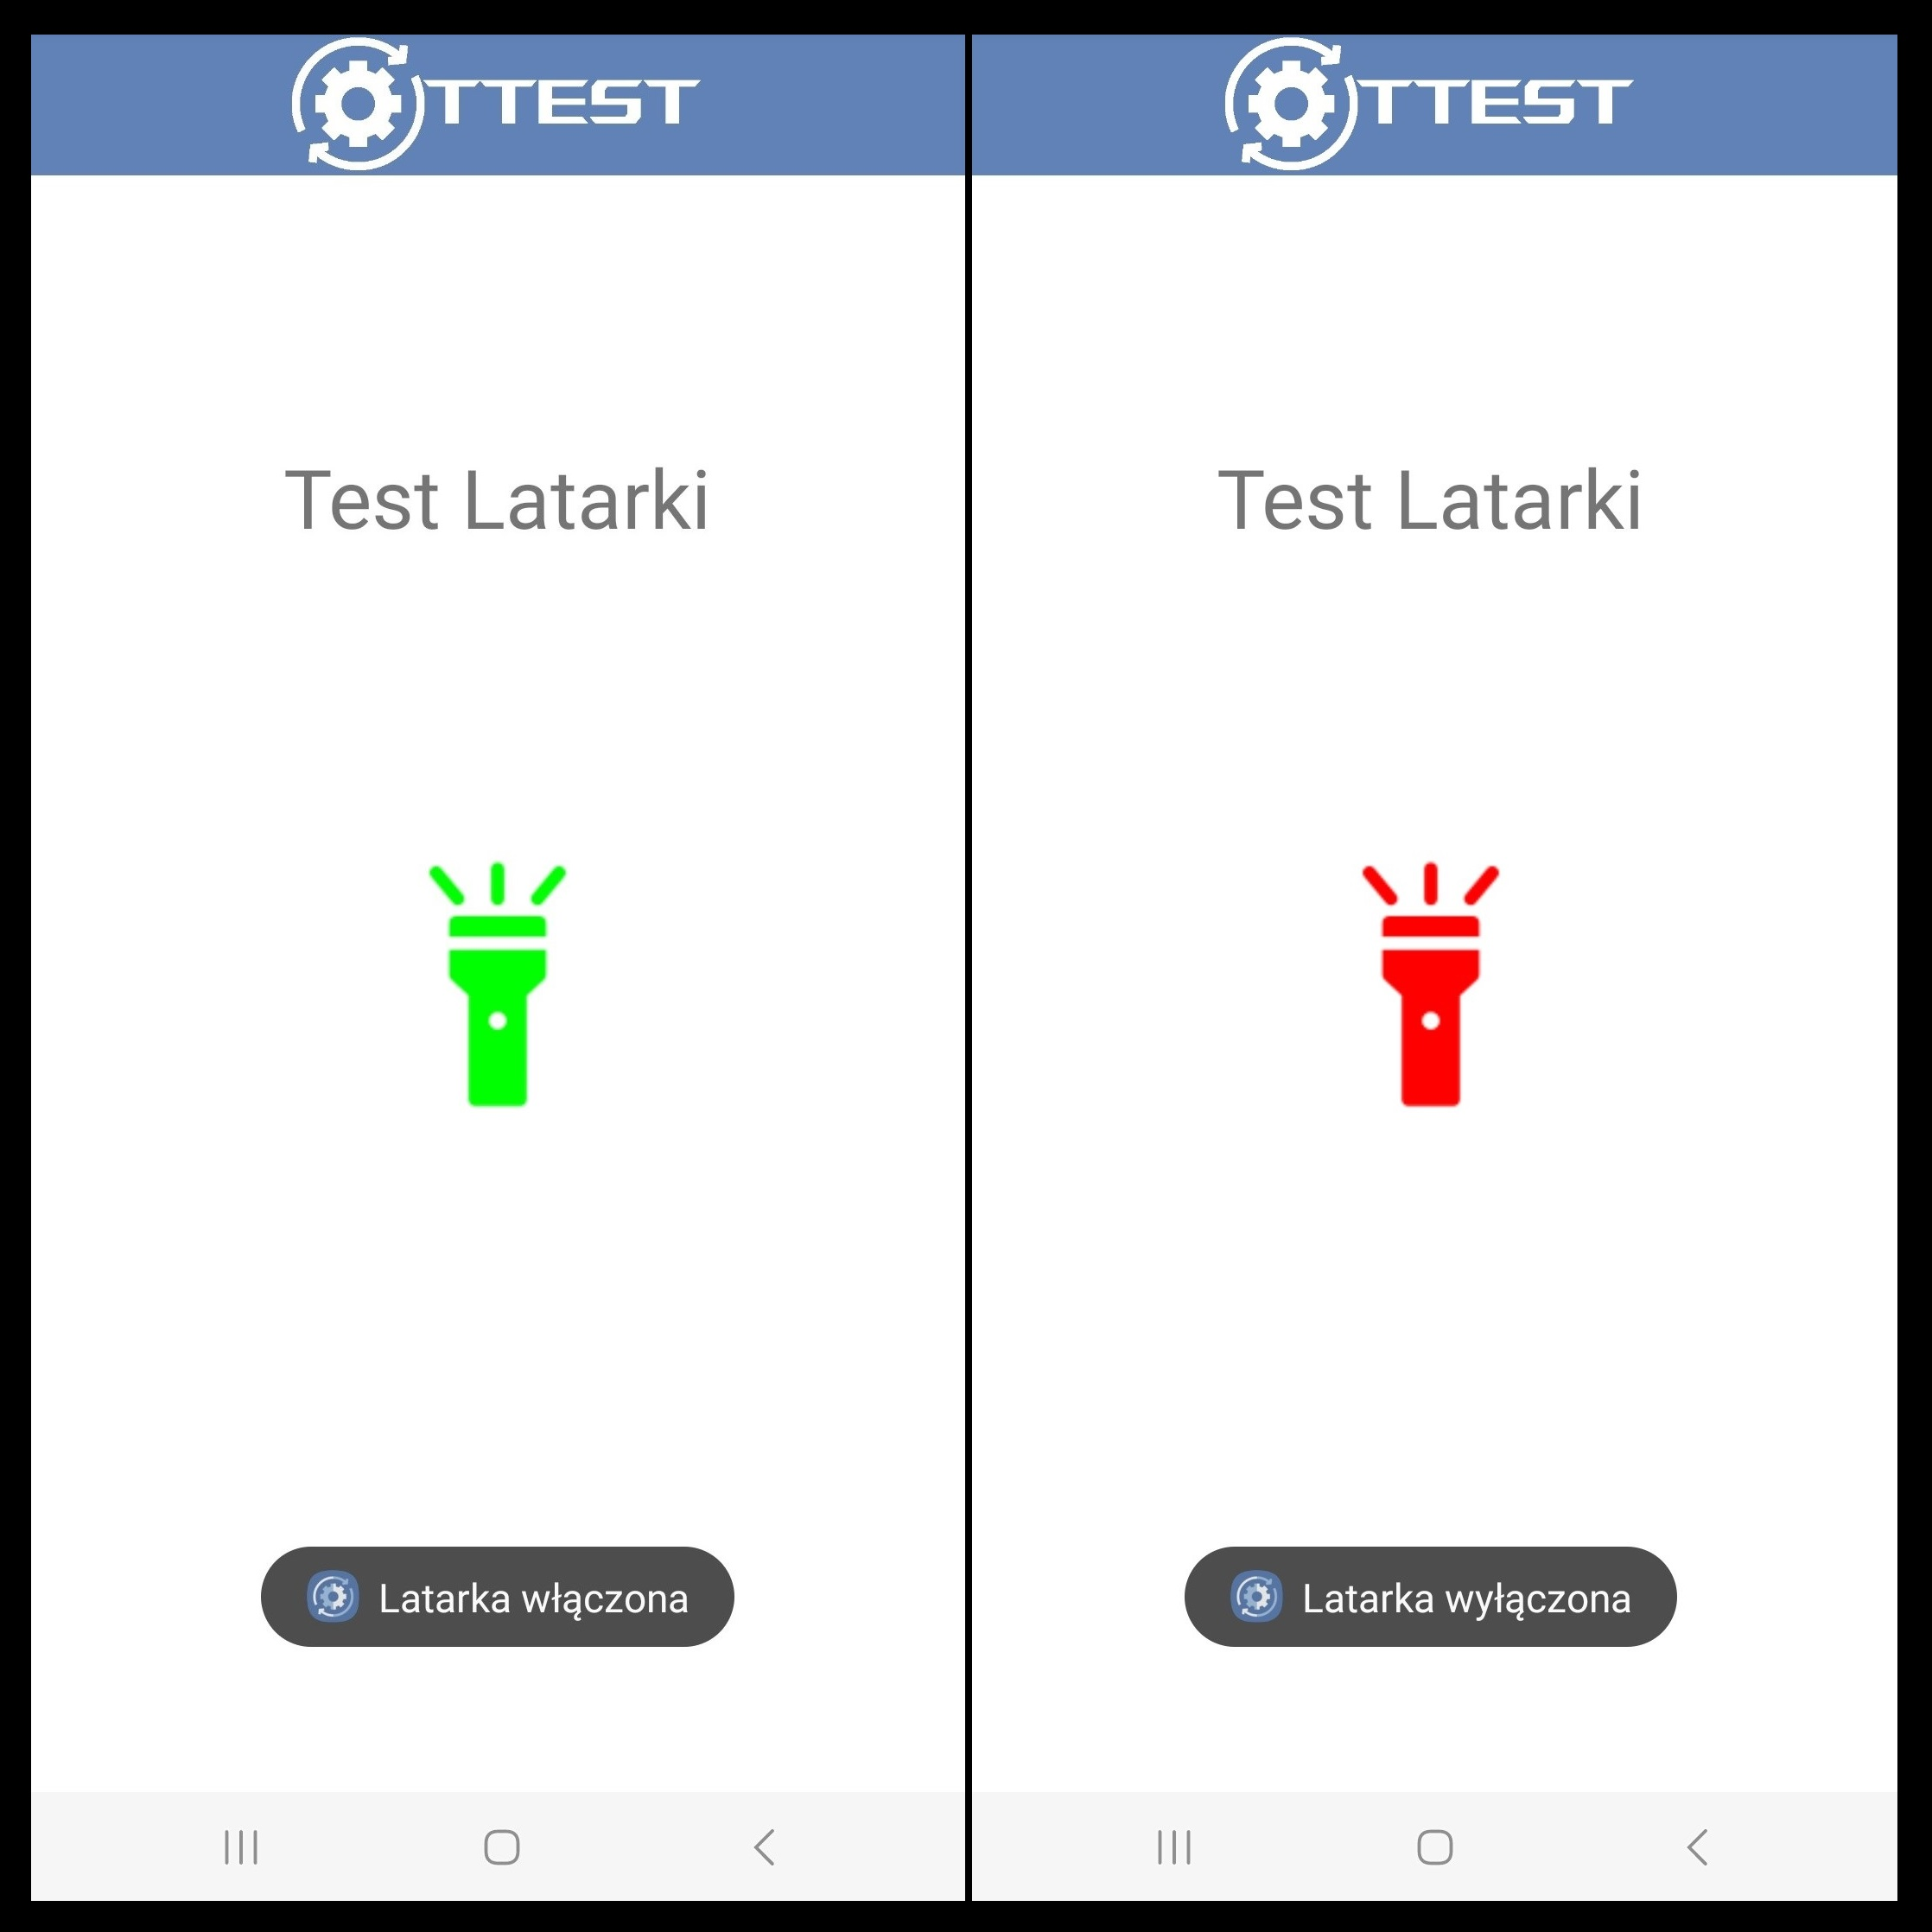
\includegraphics[angle=360, width=0.65\textwidth]{rys/punkt5/latarka.jpg}
		\caption{Przebieg testowania latarki}
		\label{rys:latarka}
	\end{center}
\end{figure}   


